\section{Project Overview}

This report consolidates the full antiship missile design into a single, closed-loop engagement. The vehicle is a solid-propellant, sea-skimming cruise missile equivalent to the Exocet/MM40 (MANSUP) class. Starting from a preliminary sizing, the model is carried through DATCOM aerodynamics, a variable-mass 6DOF model, gain-scheduled autopilots and, finally, a complete 6DOF guided flight (\texttt{GuiamentoControle.slx}).

Relative to the earlier integrated report, the guidance is no longer studied in a decoupled horizontal point-mass projection. It is now flown in the true vertical-plus-lateral geometry, with proportional navigation projected onto the body axes and gravity compensation. Because the projections changed, the numerical results changed as well: the headline figures below come from the current closed-loop 6DOF model.

\subsection{Concept of Operations (CONOPS)}

\begin{table}[H]
\centering
\caption{Flight profile of the sea-skimming engagement.}
\begin{tabular}{p{0.20\textwidth}p{0.72\textwidth}}
\toprule
Phase & What happens \\
\midrule
Launch and boost & Booster accelerates to $\approx$ Mach $0.93$ in $4~\text{s}$; the missile descends to skim altitude. Fins locked during the first $T_{Trav}$. \\
Low-level cruise & Sustainer holds Mach $0.90$; altitude control keeps $\approx 10$--$26~\text{m}$, below the radar horizon. \\
Terminal (homing) & Seeker locks the target; proportional navigation commands the intercept. \\
Bingo & Proximity fuze detonates at $<20~\text{m}$ from the ship. \\
\bottomrule
\end{tabular}
\end{table}

\subsection{Engineering Chain}

The missile is defined once and that definition feeds every stage consistently. The single source of truth is \texttt{00\_Comum/DadosMissilComum.m} and \texttt{DadosCGInerciaComum.m}; each stage folder calls them through a forwarder.

\[
\text{Sizing} \rightarrow
\text{Aerodynamics (DATCOM)} \rightarrow
\text{6DOF dynamics} \rightarrow
\text{Autopilots} \rightarrow
\text{Guidance \& Control}
\]

The final stages are integrated in a single Simulink model, \texttt{GuiamentoControle.slx}, whose top level is shown in Figure~\ref{fig:simulink_full}. It closes the loop between six blocks: the \emph{Target} (the ship), the \emph{Seeker} (AD, which measures the line-of-sight geometry), \emph{Guidance \& Control} (cruise attitude control and terminal proportional navigation), the \emph{Autopilot} (which drives the fins), the \emph{6DOF Dynamics} (the variable-mass rigid-body airframe), and \emph{Flight Termination} (which stops the run on bingo, sea impact, target overrun or low speed). Each block feeds the next, and the complete missile state is fed back every integration step.

\begin{figure}[H]
\centering
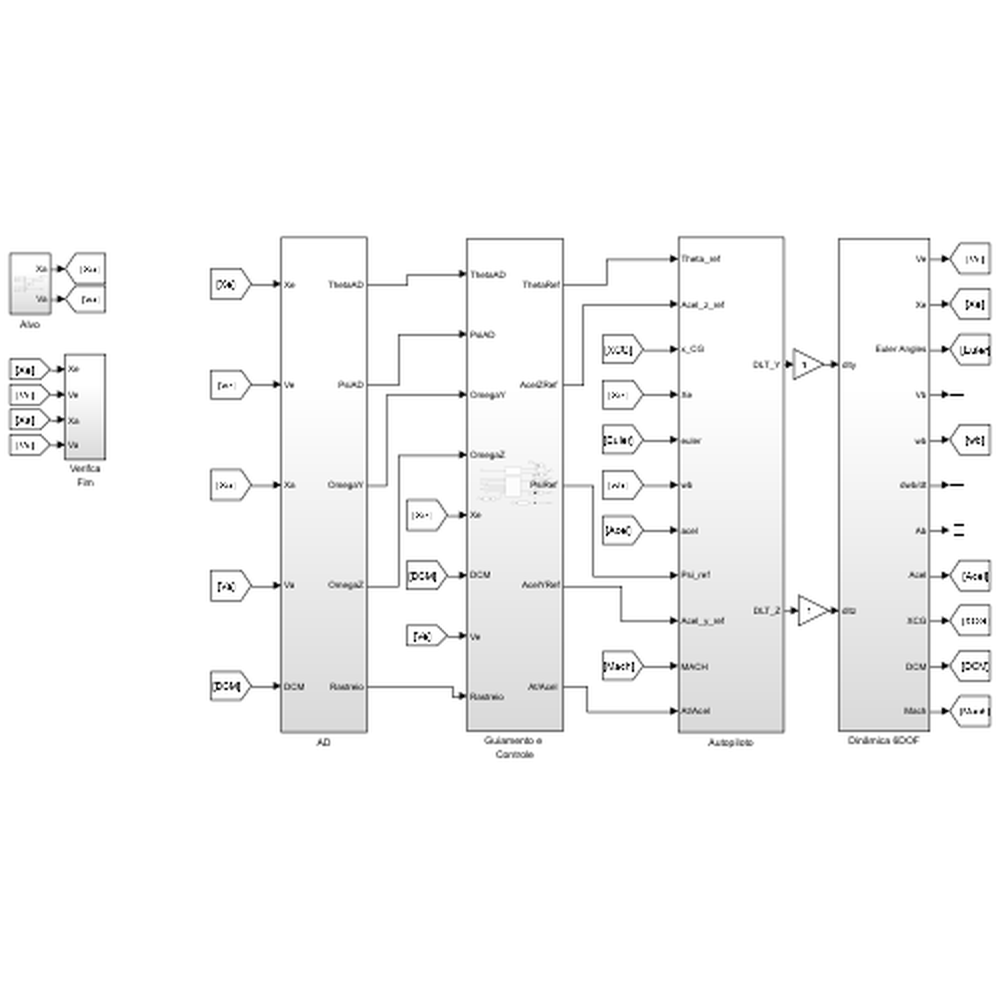
\includegraphics[width=0.98\textwidth]{figures/simulink_model_full.png}
\caption{Top level of the integrated closed-loop Simulink model \texttt{GuiamentoControle.slx}: Target, Seeker (AD), Guidance \& Control, Autopilot, 6DOF Dynamics and Flight Termination.}
\label{fig:simulink_full}
\end{figure}

\subsection{Design Requirements}

\begin{table}[H]
\centering
\caption{Preliminary design requirements.}
\begin{tabular}{p{0.30\textwidth}p{0.12\textwidth}p{0.16\textwidth}p{0.30\textwidth}}
\toprule
Parameter & Symbol & Value & Role \\
\midrule
Length & $L$ & $5.79~\text{m}$ & airframe geometry \\
Diameter & $D_{ref}$ & $0.35~\text{m}$ & reference area \\
Range & --- & $70~\text{km}$ & operational requirement \\
Cruise speed & --- & Mach $0.90$ & high-subsonic limit (avoids shock wave) \\
Warhead & CDG & $165~\text{kg}$ & payload / lethality \\
Skim altitude & $H_{ref}$ & $\approx 10~\text{m}$ & stealth (sea-skim) \\
Terminal maneuver & --- & $\geq 5g$ & intercept \\
Airframe bandwidth & --- & $\geq 0.5~\text{Hz}$ & control agility \\
\bottomrule
\end{tabular}
\end{table}

Mach $0.90$ is chosen because above it the flow goes transonic: a shock wave forms, drag spikes and the missile burns fuel and loses speed. Cruising at the top of the subsonic band is the fastest possible without paying the shock-wave penalty.

\subsection{Headline Result}

The closed-loop 6DOF engagement reaches the ship with a miss distance of $17.9~\text{m}$ (below the $20~\text{m}$ fuze radius) at Mach $0.90$, $t\approx 207~\text{s}$. All requirements are satisfied and verified in simulation.
